\documentclass{article}

\usepackage[french]{babel}
\usepackage[utf8]{inputenc}
\usepackage{graphicx}
\usepackage{amssymb, amsmath, amsthm}

%%%%%%%%%%%%%%%% Lengths %%%%%%%%%%%%%%%%
\setlength{\textwidth}{15.5cm}
\setlength{\evensidemargin}{0.5cm}
\setlength{\oddsidemargin}{0.5cm}

%%%%%%%%%%%%%%%% Variables %%%%%%%%%%%%%%%%
\def\projet{3}
\def\titre{Compression d'image par la factorisation SVD}
\def\groupe{4}
\def\equipe{1}
\def\responsible{}
\def\secretary{}
\def\others{}

\begin{document}

%%%%%%%%%%%%%%%% Header %%%%%%%%%%%%%%%%
\noindent\begin{minipage}{0.98\textwidth}
	\vskip 0mm
	\noindent
	{ \begin{tabular}{p{7.5cm}}
		{\bfseries \sffamily
			Projet \projet} \\ 
		{\itshape \titre}
		\end{tabular}}
	\hfill 
	\fbox{\begin{tabular}{l}
		{~\hfill \bfseries \sffamily Groupe \groupe\ - Equipe \equipe
			\hfill~} \\[2mm] 
		Responsable : \responsible \\
		Secrétaire : \secretary \\
		Codeurs : \others
		\end{tabular}}
	\vskip 4mm ~

	~~~\parbox{0.95\textwidth}{\small \textit{Résumé~:} \sffamily
		Ce projet a pour objectif d'effectuer des transformations sur les matrices. Les trois premières parties définissent quelques 
		fonctions permettant de manipuler et de transformer des matrices normales en des matrices bidiagonales et diagonales. Ainsi, dans la dernière partie, ces 
		transformations sont utilisées dans l'algorithme de compression d'images basé sur la transformation SVD.
	}
	\vskip 1mm ~
\end{minipage}

%%%%%%%%%%%%%%%% Main part %%%%%%%%%%%%%%%%

\section{Transformations de Householder}
Le but de cette partie est de mettre en place les fonctions nécessaires pour l'utilisation des
matrices de Householder, permettant de mettre en forme certaines matrices.

\subsection{Construction d'une matrice de Householder}

Pour la matrice de Householder, on a l'équation~\ref{eq:householder_matrix},
où $H$ représente la matrice de Householder, puis $N$ un vecteur de taille $n$ et de norme euclidienne $1$.
\begin{equation}
	H = I - 2 \times N \times N^T
	\label{eq:householder_matrix}
\end{equation}

On cherche à trouver comment choisir le vecteur $N$ afin que la matrice de Householder
$H_{U,V}$ envoie $U$ sur $V$. On considère $U$ et $V$ deux vecteurs de même norme.
Si $U^T \times N = 0$, on a $U = V$ et donc $H = I$.
Sinon, on a $N$ colinéaire à $U - V$, et sa valeur est donnée par l'équation~\ref{eq:householder_n}.
\begin{equation}
	N=\pm \frac{U-V}{\|U-V\|}
	\label{eq:householder_n}
\end{equation}

On a donc implémenté une fonction \verb|householder| permettant de calculer $N$ à l'aide de l'équation~\ref{eq:householder_n}, en traitant le cas éventuel où $U$ serait égal à $V$
pour éviter une division par $0$.

Cette fonction permet d'effectuer des changements de bases pour donner des matrices plus simples.
Par exemple, on peut choisir un vecteur $V$ ne contenant qu'une seule valeur non-nulle, la norme de $U$ pour que les deux vecteurs aient la même norme, 
et donc on a la matrice de passage pour le vecteur $U$ associé. C'est d'ailleurs ce que nous utilisons dans les parties suivantes.

\subsection{Produits avec une matrice de Householder}

Ensuite, on a cherché à écrire une fonction optimisée \verb|vector_product| qui calcule le produit d'une matrice de Householder par un vecteur.
En utilisant la formule \ref{eq:householder_matrix}, et par produit avec une matrice colonne $X$, on a l'équation~\ref{eq:vector_product}.
On remarque la présence du produit scalaire $N^T \times X$, ainsi le calcul de $H \times X$ se fait en $\mathcal{O}(n)$ au lieu de $\mathcal{O}(n^2)$.

\begin{equation}
	H \times X = X - 2 \times N \times \underbrace{N^T \times X}_{scalaire}
	\label{eq:vector_product}
\end{equation}

Pour le produit entre une matrice de Householder et un ensemble de vecteurs, nous avons décidé de représenter l'ensemble de vecteurs comme une matrice.
Cette matrice contient alors des vecteurs entre une colonne \verb|start| et une colonne \verb|end|, et des vecteurs nuls pour le reste.

On a donc créé deux fonctions, \verb|matrix_product_left| et \verb|matrix_product_right|, qui toutes deux utilisent le même principe avec le produit scalaire.

La complexité de ces deux fonctions est de $\mathcal{O}(n^2)$, puisqu'on effectue un produit scalaire sur $n$ vecteurs, 
ce qui est bien meilleur qu'un produit matriciel classique de complexité $\mathcal{O}(n^3)$.
\label{sec1}

\section{Mise sous forme bidiagonale}
Nous voulons transformer la matrice $A$ en une matrice bidiagonale en utilisant les fonctions \verb|compute_Q1| et \verb|compute_Q2|.
En fait, les matrices $Q_1$ et $Q_2$ annulent les éléments en dessous de la diagonale et au-dessus de la première diagonale supérieure de la matrice $A$, par itérations.

Ces fonctions font appel à la fonction \verb|householder|, qui est appelée sur des sous-matrices de la matrice de départ, pour obtenir la matrice bidiagonale.

En fait, on résout par étapes l'équation \ref{eq:bidiagonalize}, avec $BD$ une matrice bidiagonale, et $Q_{left}$ et $Q_{right}$ des matrices obtenues,
avec respectivement des produits des résultats de \verb|compute_Q1| et \verb|compute_Q2|.

\begin{equation}
	Q_{left} \times BD \times Q_{right} = A
	\label{eq:bidiagonalize}
\end{equation}

La fonction \verb|bidiagonalize| renvoie alors ces matrices $Q_{left}$, $BD$ et $Q_{right}$.
Pour montrer que cette fonction renvoie mathématiquement le bon résultat, il est nécessaire de prouver que les matrices $Q_1$ et $Q_2$ sont bien orthogonales et symétriques.

\bigbreak
\noindent\textbf{Démonstration :}
Prouvons d'abord que ces matrices sont orthogonales.
	Elles sont construites à partir de l'identité, et un bloc est modifié sur la diagonale pour y placer une matrice de Householder.
	Il suffit donc de montrer que les matrices de Householder sont bien orthogonales :
	\begin{align*}
		H &= I - 2 \times N \times N^T\\
		\Leftrightarrow H \times H^T &= (I - 2 \times N \times N^T) \times (I - 2 \times N \times N^T)\\
		\Leftrightarrow H \times H^T &= I - 4 \times N \times N^T + 4 \times N \times \underbrace{N^T \times N}_{= 1} \times N^T = I
	\end{align*}
	
	Ainsi, $H$ est bien orthogonale, et donc par produits par blocs dans les matrices, les matrices $Q_1$ et $Q_2$ sont orthogonales.
	
	Comme $N \times N^T$ est symétrique, alors $H = I - 2 \times N \times N^T$ aussi, et comme $H$ est insérée sur la diagonale d'une matrice carrée, 
	alors la matrice globale (par exemple $Q_1$) est nécessairement symétrique.
	Ainsi, $Q_1$ et $Q_2$ sont symétriques.
\qedsymbol
\bigbreak

Maintenant, il reste à montrer que l'équation~\ref{eq:bidiagonalize} reste vérifiée à chaque itération.

\bigbreak
\noindent\textbf{Démonstration :}
Montrons qu'à chaque itération, on conserve l'égalité $Q_{left} \times BD \times Q_{right} = A$, avec $Q_{left}$ et $Q_{right}$ des matrices orthogonales.

	\medbreak\noindent
	\textbf{Initialisation :} Pour commencer, on a $Q_{left} = I$, $Q_{right} = I$ et $BD = A$. 
	Nécessairement, on a bien $Q_{left} \times BD \times Q_{right} = A$, avec $Q_{left}$ et $Q_{right}$ orthogonales.

	\medbreak\noindent
	\textbf{Hérédité :} Soit $k$ un entier dans $[|0, n - 1|]$. Supposons que l'invariant soit vérifié à la fin de l'itération $k$.
	Montrons alors que l'égalité reste vérifiée pour l'itération $k + 1$.

	L'algorithme consiste à multiplier $Q_{left}$ à droite par $Q_1$, puis $Q_{right}$ à gauche par $Q_2$, et enfin multiplier $BD$ à gauche par $Q_1$ et à droite par $Q_2$.

	Les matrices $Q_{left}$ et $Q_{right}$ sont des matrices orthogonales par hypothèse, et les matrices $Q_1$ et $Q_2$ le sont aussi d'après la démonstration qui précède.
	En utilisant l'hypothèse de récurrence, on a le résultat attendu :
	\begin{equation*}
		Q_{left} \times Q_1 \times Q_1 \times BD \times Q_2 \times Q_2 \times Q_{right} = Q_{left} \times BD \times Q_{right} = A
	\end{equation*}

	En effet, $Q_1$ et $Q_2$ sont orthogonales et symétriques d'après la preuve précédente, donc elles sont auto-inverses : $Q_1 = Q_1^T = Q_1^{-1}$ et $Q_2 = Q_2^T = Q_2^{-1}$,
	ce qui donne $Q_1 \times Q_1 = I$ et $Q_2 \times Q_2 = I$.

	Par produit de matrices orthogonales, $Q_{left}$ et $Q_{right}$ restent orthogonales : l'hérédité est prouvée.

	\medbreak\noindent
	\textbf{Conclusion :} $Q_{left} \times BD \times Q_{right} = A$, l'invariant est donc vérifié.
\qedsymbol
\bigbreak\label{sec2}

\section{Implémentation de la tranformation QR et de la SVD}
Dans cette partie, nous allons transformer une matrice bidiagonale $BD$ en une matrice diagonale~$S$ par une méthode itérative,
puis créer une fonction \verb|SVD| à partir des fonctions déjà créées.

\subsection{Transformations QR}

\bigbreak
\noindent\textbf{Démonstration :}
Montrons qu'à chaque tour de boucle, on conserve l'égalité $U \times S \times V = BD$, avec $U$ et $V$ des matrices orthogonales.
	
	\medbreak\noindent
	\textbf{Initialisation :} Pour commencer, on a $U = I$, $V = I$ et $S = BD$. 
	Nécessairement, on a bien $U \times S \times V = BD$, avec $U$ et $V$ orthogonales.

	\medbreak\noindent
	\textbf{Hérédité :} Soit $k$ un entier dans $[|0, N_{max} - 1|]$. Supposons que l'invariant soit vérifié à la fin de l'itération $k$.
	Montrons alors que l'égalité reste vérifiée pour l'itération $k + 1$.

	L'algorithme consiste à multiplier $U$ à droite par $Q_2$, puis $V$ à gauche par $Q_1^T$, 
	et enfin remplacer $S$ par $R_2$.

	Les matrices $U$ et $V$ sont des matrices orthogonales par hypothèse, et les matrices $Q_1$ et $Q_2$ le sont aussi puisqu'il s'agit d'une décomposition QR,
	donc on a $Q_1 \times Q_1^T = I$ et $Q_2 \times Q_2^T = I$.

	On a les égalités suivantes : $Q_1 \times R_1 = S^T$, et $Q_2 \times R_2 = R_1^T$
	Comme $Q_2$ est orthogonale, et en utilisant que $(A \times B)^T = B^T \times A^T$, on a $R_2 = Q_2^T \times R_1^T$, et donc $R2 = Q_2^T \times S \times Q_1$.

	En utilisant l'hypothèse de récurrence, on a bien le résultat recherché :
	\begin{equation*}
		U \times Q_2 \times R_2 \times Q_1^T \times V = U \times \underbrace{Q_2 \times Q_2^T}_{= I} \times S \times \underbrace{Q_1 \times Q_1^T}_{= I} \times V = U \times S \times V = BD
	\end{equation*}
	Par produit de matrices orthogonales, $U$ et $V$ restent orthogonales. 
	Ainsi, l'hérédité est prouvée.

	\medbreak\noindent
	\textbf{Conclusion :} $U \times S \times V = BD$.
\qedsymbol
\bigbreak

\bigbreak
\noindent\textbf{Démonstration :}
Montrons qu'à chaque tour de boucle les matrices $S$, $R_1$ et $R_2$ sont bidiagonales.

	\medbreak\noindent
	\textbf{Initialisation :} Au début, la matrice $S$ est une copie de la matrice bidiagonale $BD$, et les matrices $R_1$ et $R_2$ sont vides. 
	L'initialisation est donc vérifiée.

	\medbreak\noindent
	\textbf{Hérédité :} Soit $k \in [|0, N_{max} - 1|]$. Supposons que la proposition soit vérifiée à l'itération $k$.
	Montrons alors qu'elle reste vérifiée pour l'itération $k + 1$.

	La matrice $R_1$ est mise à jour à partir de la matrice $S$ de l'itération $k$ en utilisant la \textit{factorisation~QR} ($S^T = Q_1 \times R_1$). Or la \textit{factorisation QR} 
	conserve la structure des matrices, par conséquent $R_1$ est aussi bidiagonale. De la même manière, on montre que $R_2$ est aussi bidiagonale 
	puisqu'elle est obtenue par \textit{factorisation QR} sur la matrice $R_1$ de l'itération $k + 1$ ($R_1^T = Q_2 \times R_2$).

	Ensuite, la matrice $S$ est égale à $R_2$ de l'itération $k + 1$, elle est donc bidiagonale.
	Ainsi, l'hérédité est prouvée.

	\medbreak\noindent
	\textbf{Conclusion :} Les matrices $S$, $R_1$ et $R_2$ restent bidiagonales à chaque itération.
\qedsymbol
\bigbreak

La fonction \verb|QR| a une complexité de l'ordre de $\mathcal{O}(n^3)$.
En effet, on utilise dans la boucle les fonctions \verb|matrix_product_right| et \verb|matrix_product_left|, qui ont des complexités de l'ordre de $\mathcal{O}(n^2)$.

\subsection{Algorithme de la factorisation SVD}
Avec les fonctions que nous avons implémentées, il est possible d'effectuer une factorisation SVD.
Il suffit d'appliquer ceci : \verb|bidiagonalize(A)|, ce qui donne $A = Q_{left} \times BD \times Q_{right}$.
Ensuite, on applique la seconde fonction sur $BD$ : \verb|U, S, V = diagonalize(BD)|, qui donne $BD = U \times S \times V$.
L'équation \ref{eq:svd} montre alors la décomposition de $A$ en matrice diagonale.

\begin{equation}
	A = Q_{left} \times U \times S \times V \times Q_{right}
	\label{eq:svd}
\end{equation}

Pour compléter notre fonction \verb|SVD|, nous avons ordonné les valeurs sur la diagonale de la matrice $S$ de manière décroissante, 
en effectuant des permutations à la fois sur les lignes de la matrice $U$ et sur celles de $S$.

Comme la fonction \verb|QR| est appelée à l'intérieur de la boucle présente dans la fonction \verb|diagonalize|, qui fait partie de la fonction \verb|SVD|,
la complexité de la fonction \verb|SVD| est de l'ordre de $\mathcal{O}(n^4)$.
Même si cette complexité est très élevée, elle permet d'avoir une stabilité numérique importante.\label{sec3}

\section{Application de la SVD à la compression d'image}
Pour terminer, dans cette partie, nous allons appliquer les transformations de matrices vues dans les parties 2 et 3 à 
l'algorithme de compression d'image par factorisation SVD.\\

On cherche à utiliser la compression SVD sur une image contenant 3 composantes : rouge, vert et bleu.
Pour cela, on récupère une matrice d'intensité pour chacune des couleurs, ce qui permet d'appliquer la compression SVD sur chacune des composantes.

Notons $R$, $G$ et $B$ les matrices d'intensités correspondant aux 3 composantes.
Notons $U_r$, $V_r$, $S_r$ les matrices obtenues pour $R$,
$U_g$, $V_g$, $S_g$ les matrices obtenues pour $G$ puis
$U_b$, $V_b$, $S_b$ les matrices obtenues pour $B$.
On a alors $R = U_r \times S_r \times V_r$, $G = U_g \times S_g \times V_g$ et enfin
$B = U_b \times S_b \times V_b$.
\bigbreak
Pour obtenir une compression au rang $r$ sur toutes les composantes, 
on annule tous les termes diagonaux de $S_r$, $S_g$ et $S_b$ d'indices 
strictement supérieurs à $r$, et inférieurs à $min(m, n)$.
En réalité, ce calcul en entraîne un autre : comme on perd de l'information, il se peut que les valeurs dans la nouvelle matrice $U \times S \times V$ deviennent inférieures à 0 ou supérieures à 1 
(ou 255 dans le cas où l'on raisonne sur des entiers).
La solution a donc été de borner les valeurs, et donc de les ramener aux bords du domaine si elles dépassaient du bord.
\bigbreak
En faisant cela, on perd de l'information sur l'image, mais la quantité de données stockées est moins grande.
En effet, pour stocker l'image, au lieu de stocker $n \times m$ données, il suffit de stocker 
les parties de $U$ et $V$ qui n'entraînent pas de produits nuls avec les matrices $S$ (ce qui donne des matrices de taille $k \times m$ et $n \times k$)
en plus des diagonales des matrices $S$ (seule la diagonale suffit puisque ce sont des matrices diagonales).

Notons qu'en enregistrant par exemple $U$ et $S \times V$, on peut éviter d'enregistrer la diagonale de $S$, ce qui donnerait exactement deux matrices de tailles $k \times m$ et $n \times k$.
C'est ce que l'on considère dans la suite.
Dans ce cas, on stocke $3 \times r \times (n + m)$ valeurs.
Cette taille est généralement inférieure à la taille de départ, mais à partir d'une certain rang $r_{lim}$, la compression perd de son sens, pour $r_{lim} = \frac{n \times m}{n + m}$.
\bigbreak

Nous avons tracé la norme de la différence de l'image générée à l'image de départ, en échelle logarithmique en figure~\ref{fig:p4-dist}. De toute évidence, dès que le rang atteint $min(n, m)$,
la différence est nulle.
Nous pouvons remarquer que même avec un rang de compression assez faible, on peut garder un écart très faible à l'image originale.

On peut voir le rang $r_{lim}$ à partir duquel la compression n'est plus intéressante en termes de stockage. Pour ce rang, l'image semble très similaire à celle de base,
mais par exemple pour une compression de rang 110, et le résultat est très similaire, cette méthode est donc intéressante en ce qui concerne le stockage.

\begin{figure}[htbp]
	\centering
	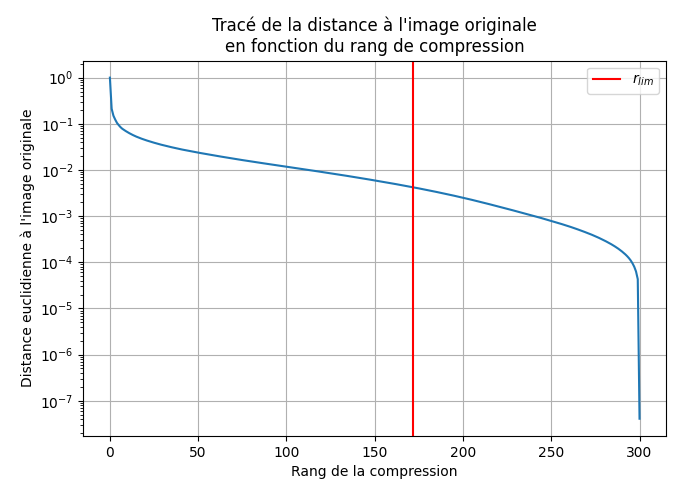
\includegraphics[width=0.65\textwidth]{res/part-4-dist.png}
	\caption{Tracé de l'efficacité de la compression (avec l'image fournie).} 
	\label{fig:p4-dist}
\end{figure}\label{sec4}

\end{document}